%=====================================================================
%  Póster A1 vertical — Proyecto Final I302
%  Estadificación del sueño con SmartWatch (BiLSTM · contexto inter-época)
%  Autores: A. A. Pereyra & A. Patruno — Universidad de San Andrés
%
%  Compilar:  pdflatex poster.tex   (dos veces)
%  Requiere las figuras en ../report/figures/
%=====================================================================
\documentclass[25pt, a1paper, portrait, margin=14mm, innermargin=10mm,
               blockverticalspace=8mm, colspace=10mm, subcolspace=6mm]{tikzposter}

\usepackage[utf8]{inputenc}
\usepackage[T1]{fontenc}
\usepackage[spanish,es-noshorthands]{babel}
\usepackage{amsmath,amssymb}
\usepackage{graphicx}
\usepackage{booktabs}
\usepackage{colortbl}
\usepackage{array}
\usepackage{tikz}

\tikzposterlatexaffectionproofoff   % quita el sello "LaTeX TikZposter"

%--------------------------------------------------------------------
%  Paleta (3 colores, como pide la guía): midnight · ivory · ámbar
%--------------------------------------------------------------------
\definecolor{midnight}{HTML}{0E1330}
\definecolor{ivory}{HTML}{F7F4EE}
\definecolor{amber}{HTML}{E8912A}
\definecolor{ambersoft}{HTML}{F6C27A}
\definecolor{ink}{HTML}{141A33}
\definecolor{mutedc}{HTML}{5C6284}
\definecolor{tint}{HTML}{EEEADF}
\definecolor{sWake}{HTML}{E8912A}\definecolor{sN1}{HTML}{6E97C9}
\definecolor{sN2}{HTML}{3F63A6}\definecolor{sN3}{HTML}{233A73}
\definecolor{sREM}{HTML}{8E6FB0}

%--------------------------------------------------------------------
%  Estilo: fondo ivory, título del póster midnight, bloques con
%  barra de título midnight y cuerpo blanco.
%--------------------------------------------------------------------
\usetheme{Default}
\usecolorstyle{Germany}
\colorlet{backgroundcolor}{ivory}
\colorlet{framecolor}{ivory}
\colorlet{titlefgcolor}{ivory}
\colorlet{titlebgcolor}{midnight}
\colorlet{blocktitlebgcolor}{midnight}
\colorlet{blocktitlefgcolor}{ivory}
\colorlet{blockbodybgcolor}{white}
\colorlet{blockbodyfgcolor}{ink}
\useblockstyle{Default}

% Encabezado grande dentro del cuerpo de un bloque
\newcommand{\lead}[1]{{\color{ink}\bfseries\Large #1}\par\vspace{2mm}}
\newcommand{\pnote}[1]{{\small\color{mutedc} #1}}

% Bloque con cuerpo ámbar (para la franja de resultado)
\newenvironment{amberblock}{%
  \colorlet{blockbodybgcolor}{amber}\colorlet{blockbodyfgcolor}{midnight}%
  \colorlet{blocktitlebgcolor}{amber}\colorlet{blocktitlefgcolor}{midnight}}{}
% Bloque con cuerpo midnight (para hallazgo / cierre)
\newenvironment{darkblock}{%
  \colorlet{blockbodybgcolor}{midnight}\colorlet{blockbodyfgcolor}{ivory}%
  \colorlet{blocktitlebgcolor}{midnight}\colorlet{blocktitlefgcolor}{ambersoft}}{}

%--------------------------------------------------------------------
\title{\parbox{0.92\linewidth}{El contexto entre épocas manda:\\[2mm]
       estadificación del sueño desde un SmartWatch}}
\author{Agustín A. Pereyra \quad\textbullet\quad Agustín Patruno}
\institute{Departamento de Ingeniería — Universidad de San Andrés, Buenos Aires\\
           \texttt{apereyra@udesa.edu.ar} \quad\textbullet\quad \texttt{apatruno@udesa.edu.ar}}

\begin{document}
\maketitle[titletextscale=0.85, roundedcorners=0, linewidth=0pt,
           titletoblockverticalspace=8mm]

%======================= FRANJA RESULTADO ==========================
\begin{columns}\column{1}
\begin{amberblock}
\block{Resultado principal}{%
  \begin{minipage}[c]{0.26\linewidth}\centering\color{midnight}
    {\fontsize{72}{72}\selectfont\bfseries +12}\\[1mm]{\Large\bfseries pts $\kappa$}
  \end{minipage}\hfill
  \begin{minipage}[c]{0.70\linewidth}\color{midnight}\large
    Una \textbf{BiLSTM} sobre features por época ($\kappa\approx0.46$,
    $F1_{\text{macro}}\approx0.57$) supera a los baselines tabulares por
    \textbf{$\sim$12 puntos de Cohen's $\kappa$}. El factor decisivo no es el clasificador
    ni la señal cruda: es la \textbf{dependencia temporal entre épocas}.
  \end{minipage}}
\end{amberblock}
\end{columns}

%========================= CUERPO 3 COLUMNAS =======================
\begin{columns}

%------------------------------ COLUMNA 1 --------------------------
\column{0.34}

\block{El problema · De la polisomnografía a la muñeca}{%
  La estadificación del sueño —asignar una etapa a cada época de \textbf{30\,s} según el estándar
  clínico AASM— es clave para diagnosticar apnea o insomnio, pero hoy exige \textbf{polisomnografía}:
  cara, incómoda y de laboratorio. Un SmartWatch mide de forma continua y no invasiva.\par\vspace{2mm}
  \textbf{Entrada:} IHR (frecuencia cardíaca instantánea) + acelerometría triaxial de un Apple Watch.\\
  \textbf{Salida:} etapa por época — Wake · N1 · N2 · N3 · REM.\par\vspace{3mm}
  \small\textcolor{sWake}{$\blacksquare$}~Wake\quad\textcolor{sN1}{$\blacksquare$}~N1\quad
  \textcolor{sN2}{$\blacksquare$}~N2\quad\textcolor{sN3}{$\blacksquare$}~N3\quad
  \textcolor{sREM}{$\blacksquare$}~REM}

\block{Datos · 47 adultos, 253 noches (PhysioNet BIDSleep)}{%
  Etiquetas de dos fuentes: un \textbf{experto} en polisomnografía (ground-truth, AASM) y un
  dispositivo \textbf{Dreem} basado en EEG (referencia y competencia directa; acuerdo experto--Dreem
  $\kappa\approx0.72$). Clases fuertemente \textbf{desbalanceadas} — de ahí evaluar con
  $F1_{\text{macro}}$ y usar costo ponderado por clase.\par\vspace{4mm}\centering
  \begin{tikzpicture}[y=7mm]
    \foreach \i/\name/\pct/\w/\c in {%
      0/N2/37.5/6.0/sN2, 1/REM/25.9/4.14/sREM, 2/N3/18.5/2.96/sN3,
      3/Wake/11.0/1.76/sWake, 4/N1/7.1/1.14/sN1}{
      \node[left] at (0,-\i){\small\name};
      \fill[\c] (0.4,-\i-0.2) rectangle (0.4+\w,-\i+0.2);
      \node[right] at (0.4+\w,-\i){\small\color{mutedc}\pct\%};}
  \end{tikzpicture}}

\block{Limpieza de señal · pipeline estricto y reproducible}{%
  \begin{itemize}\setlength\itemsep{1mm}
    \item Corrección de desalineación temporal (zona local vs. Unix UTC) y filas corruptas.
    \item \textbf{Ventana válida} = rango etiquetado $\cap$ IHR continuo $\cap$ acelerometría continua.
    \item \emph{Gaps} internos: recorte de cola o descarte; dropouts dispersos filtrados por época.
    \item Misma fuente de verdad para las 3 rutas de datos $\Rightarrow$ comparación honesta.
  \end{itemize}\vspace{2mm}\centering
  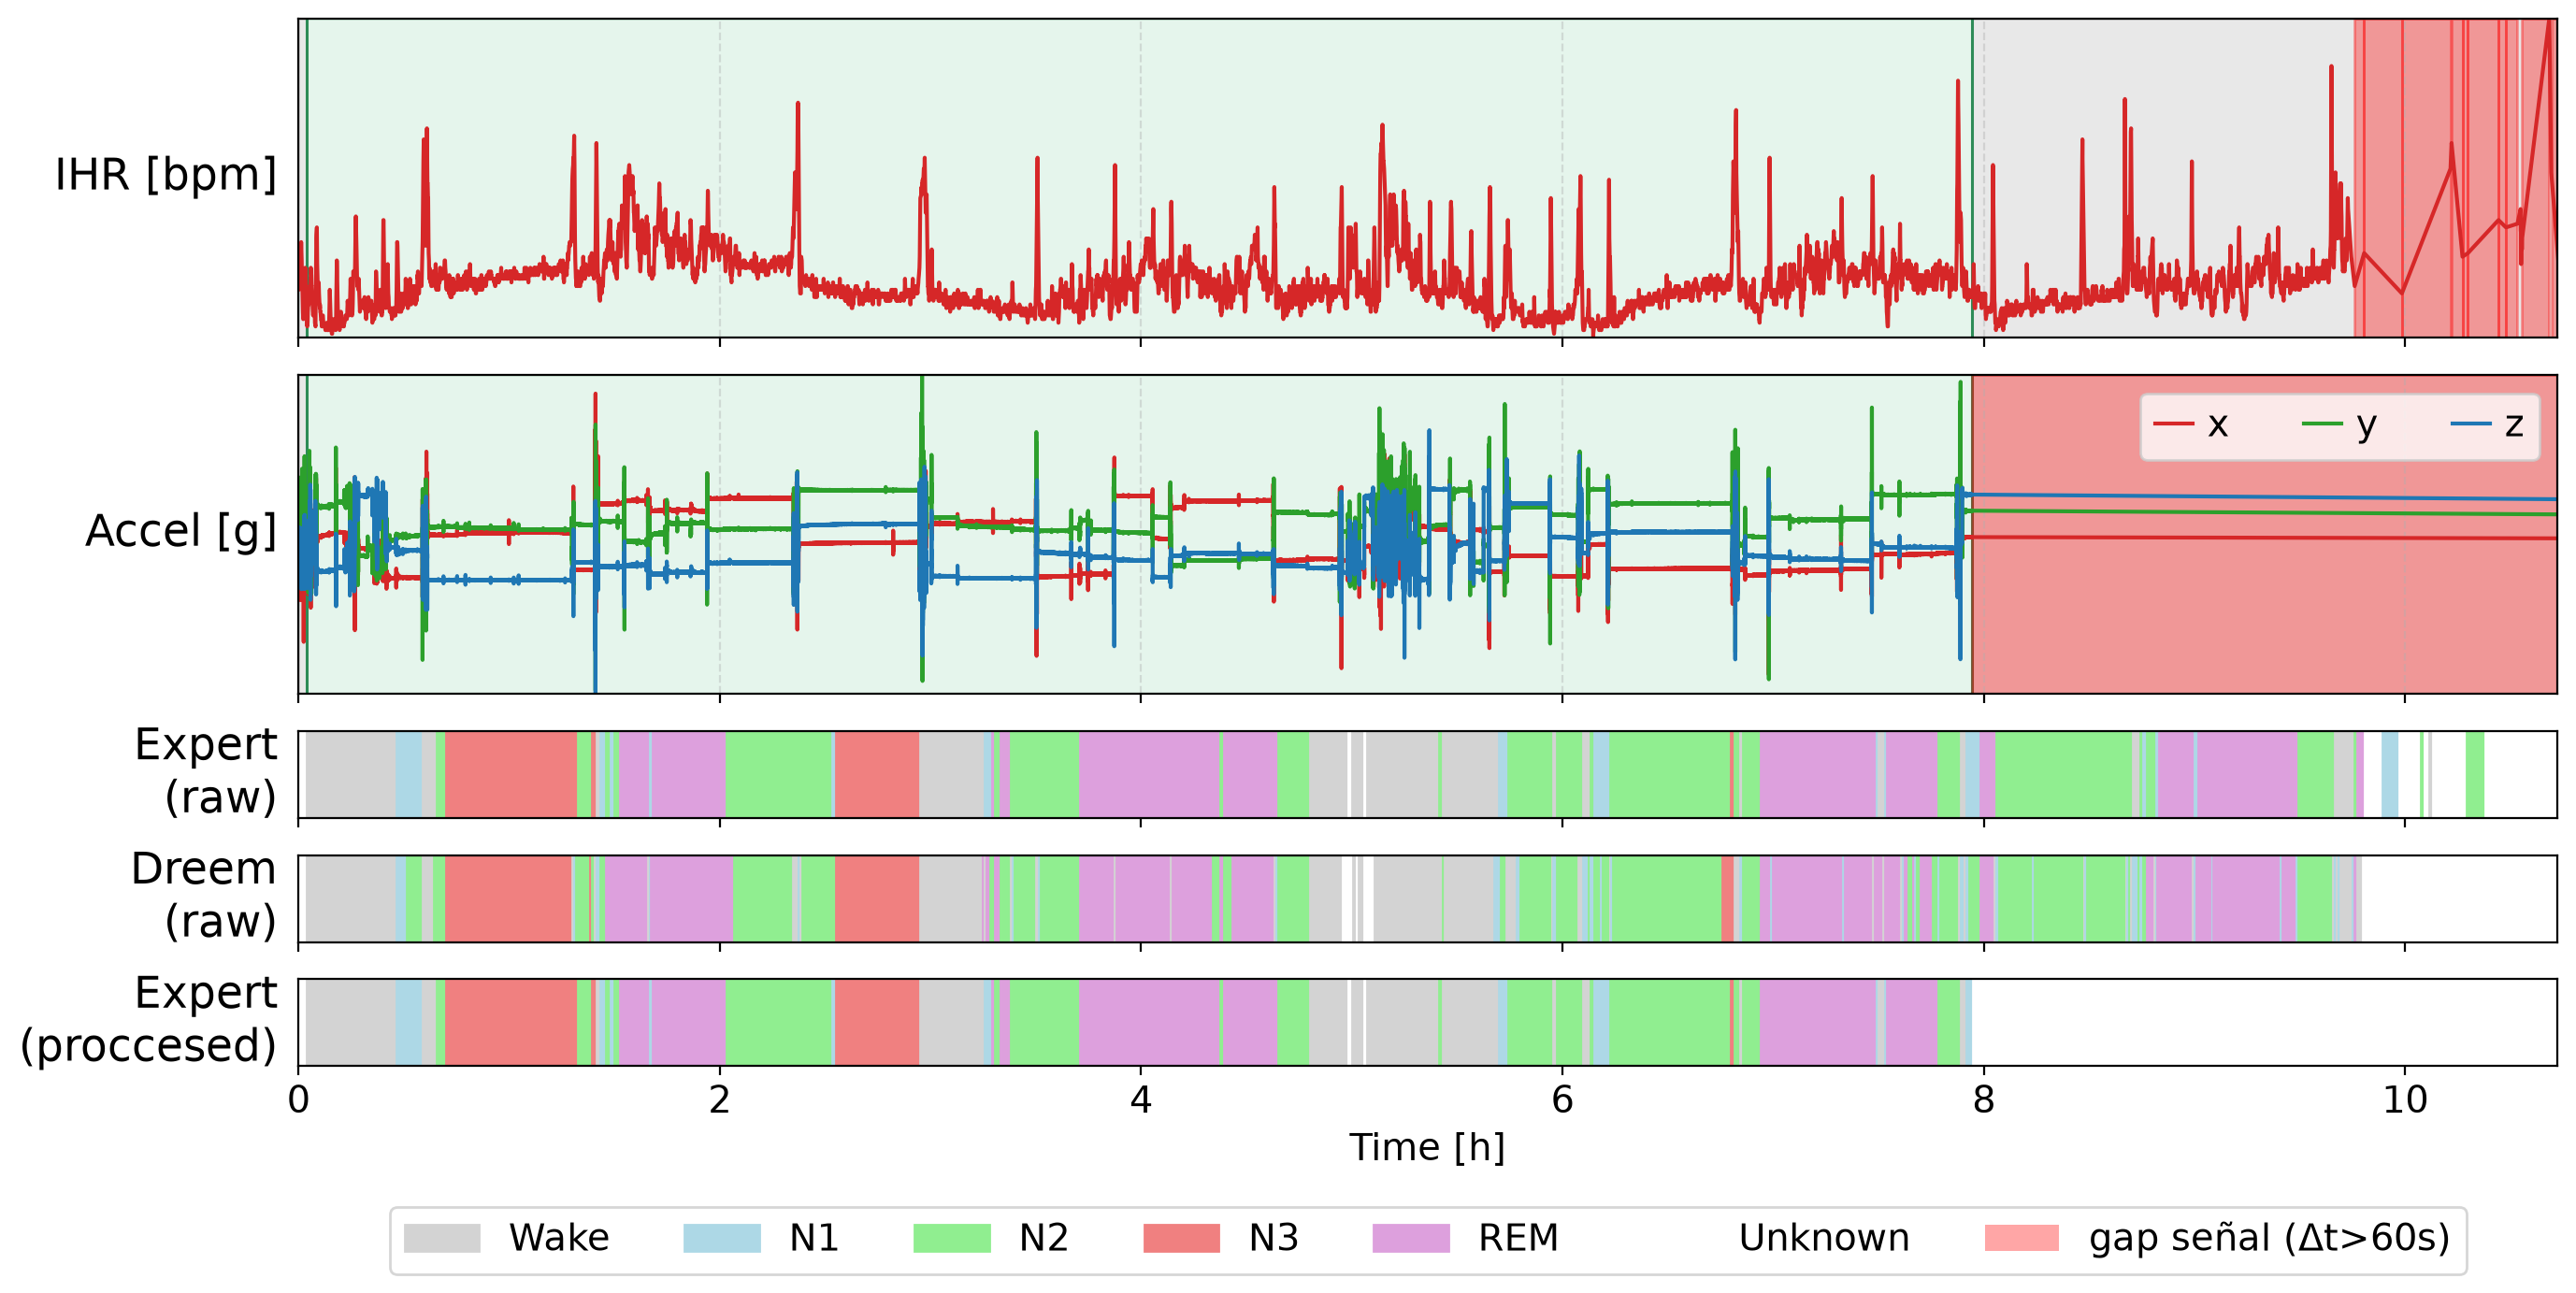
\includegraphics[width=\linewidth]{../report/figures/raw-vs-clean-20-1.png}\\[1mm]
  \pnote{\itshape Noche procesada (Paciente 20): en verde la ventana válida, en rojo la zona descartada.}}

\block{Apéndice · Autoencoder no supervisado}{%
  Un \textbf{autoencoder LSTM} comprime cada noche en un embedding por época ($L{=}32$) reconstruyendo
  las features \textbf{sin etiquetas}; un XGBoost clasifica sobre él.\par\vspace{3mm}\centering\small
  \begin{tabular}{@{}lccc@{}}\toprule
    Entrada XGBoost & $F1_M$ & $\kappa$(5cl) & $\kappa$(4cl)\\\midrule
    \rowcolor{tint}\textbf{Handcrafted (122)} & 0.47 & 0.38 & 0.39\\
    Embeddings (32) & 0.40 & 0.29 & 0.29\\
    Ambas (154) & 0.47 & 0.38 & 0.38\\\bottomrule
  \end{tabular}\par\vspace{2mm}\raggedright
  \pnote{\textbf{No:} los embeddings quedan por debajo de las handcrafted ($\Delta\kappa\approx-0.09$)
  y sumarlos no aporta. El conocimiento de dominio le gana a la representación no supervisada.}}

%------------------------------ COLUMNA 2 --------------------------
\column{0.34}

\block{Metodología · Progresión de modelos}{%
  Comparamos una progresión pensada para \textbf{aislar el aporte del contexto inter-época}:
  \par\vspace{2mm}
  \textbf{BASELINE — XGBoost \& MLP.} 122 features handcrafted por época; clasifican cada época de
  forma \textbf{aislada}.\par\vspace{1.5mm}
  {\color{amber}\textbf{GANADOR — BiLSTM} (many-to-many).} Recorre la noche entera sobre las mismas
  features $\Rightarrow$ modela la \textbf{dinámica inter-época}.\par\vspace{1.5mm}
  \textbf{HÍBRIDO — CNN1D$\to$BiLSTM.} La CNN aprende la época desde la \textbf{señal cruda}
  ($150{\times}4$); la BiLSTM la secuencia. End-to-end.\par\vspace{3mm}
  \pnote{Redes entrenadas con \textbf{cross-entropy ponderada por clase} e hiperparámetros por
  \textbf{búsqueda bayesiana (TPE / Optuna)}, optimizando $\kappa$ de validación. Split
  \textbf{por paciente} (33/7/7) para evitar leakage.}}

\block{Resultados · $\kappa$ frente al experto (5 clases)}{%
  \centering
  \begin{tikzpicture}[x=1mm,y=9mm]
    \foreach \i/\name/\val/\w/\c in {%
      0/Dreem/0.72/97/mutedc, 1/BiLSTM/0.46/62/amber, 2/Híbrido/0.36/48/sN2,
      3/MLP/0.35/47/sN1, 4/XGBoost/0.32/43/sN1}{
      \node[left] at (0,-\i){\small\name};
      \fill[tint] (2,-\i-0.33) rectangle (102,-\i+0.33);
      \fill[\c]   (2,-\i-0.33) rectangle (2+\w,-\i+0.33);
      \node[right] at (104,-\i){\small\bfseries\val};}
  \end{tikzpicture}\par\vspace{2mm}\raggedright
  \pnote{Cohen's $\kappa=(p_o-p_e)/(1-p_e)$. La BiLSTM lidera también en AUC-ROC (0.84) y AP (0.60).}}

\block{Rendimiento en test}{%
  \centering
  \begin{tabular}{@{}lcccc@{}}\toprule
    Modelo & $F1_M$ & $\kappa$(5cl) & $\kappa$(4cl) & Acc.\\\midrule
    \textit{Dreem} & \textit{0.71} & \textit{0.72} & \textit{0.80} & \textit{0.79}\\
    XGBoost & 0.44 & 0.32 & 0.34 & 0.51\\
    MLP & 0.45 & 0.35 & 0.36 & 0.53\\
    \rowcolor{tint}\textbf{BiLSTM} & \textbf{0.57} & \textbf{0.46} & \textbf{0.49} & \textbf{0.59}\\
    Híbrido & 0.48 & 0.36 & 0.39 & 0.48\\\bottomrule
  \end{tabular}\par\vspace{2mm}\raggedright
  \pnote{Al agrupar en 4 clases (Light/Deep) todas las métricas suben y el orden se mantiene: la
  ventaja del contexto no depende de la granularidad. La brecha residual con Dreem se concentra en N1
  y en las transiciones — límite intrínseco de la muñeca frente al EEG.}}

\block{Calidad del ranking · test (one-vs-rest, 5 cl.)}{%
  \centering
  \begin{tabular}{@{}lcccc@{}}\toprule
    Curva (macro) & XGB & MLP & BiLSTM & Híbr.\\\midrule
    \rowcolor{tint}\textbf{AUC-ROC} & 0.77 & 0.78 & \textbf{0.84} & 0.83\\
    AP (PR) & 0.49 & 0.50 & \textbf{0.60} & 0.57\\\bottomrule
  \end{tabular}\par\vspace{2mm}\raggedright
  \pnote{La BiLSTM lidera también en el \textbf{ranking de probabilidades}, no solo en la decisión:
  el contexto inter-época mejora la confianza asignada a cada etapa, no únicamente el umbral.}}

%------------------------------ COLUMNA 3 --------------------------
\column{0.32}

\begin{darkblock}
\block{El hallazgo · Tres evidencias convergentes}{%
  El contexto temporal \textbf{inter-época} es el factor determinante — no el modelo ni la
  representación de la señal:\par\vspace{2mm}
  {\color{amber}\textbf{1.}} La BiLSTM suma \textbf{+12 pts de $\kappa$} sobre los baselines usando
  \textbf{las mismas features}. Lo único nuevo es la secuencia.\par\vspace{1.5mm}
  {\color{amber}\textbf{2.}} Los valores \textbf{SHAP} muestran que hasta el XGBoost se apoya en
  features de contexto (posición en la noche, estadísticos móviles).\par\vspace{1.5mm}
  {\color{amber}\textbf{3.}} Una \textbf{CNN sobre señal cruda, sin contexto}, rinde \textbf{cerca del
  azar} ($\kappa\approx0.04$). Lo intra-época, solo, no alcanza.}
\end{darkblock}

\block{Resultado cualitativo · una noche reconstruida}{%
  \centering
  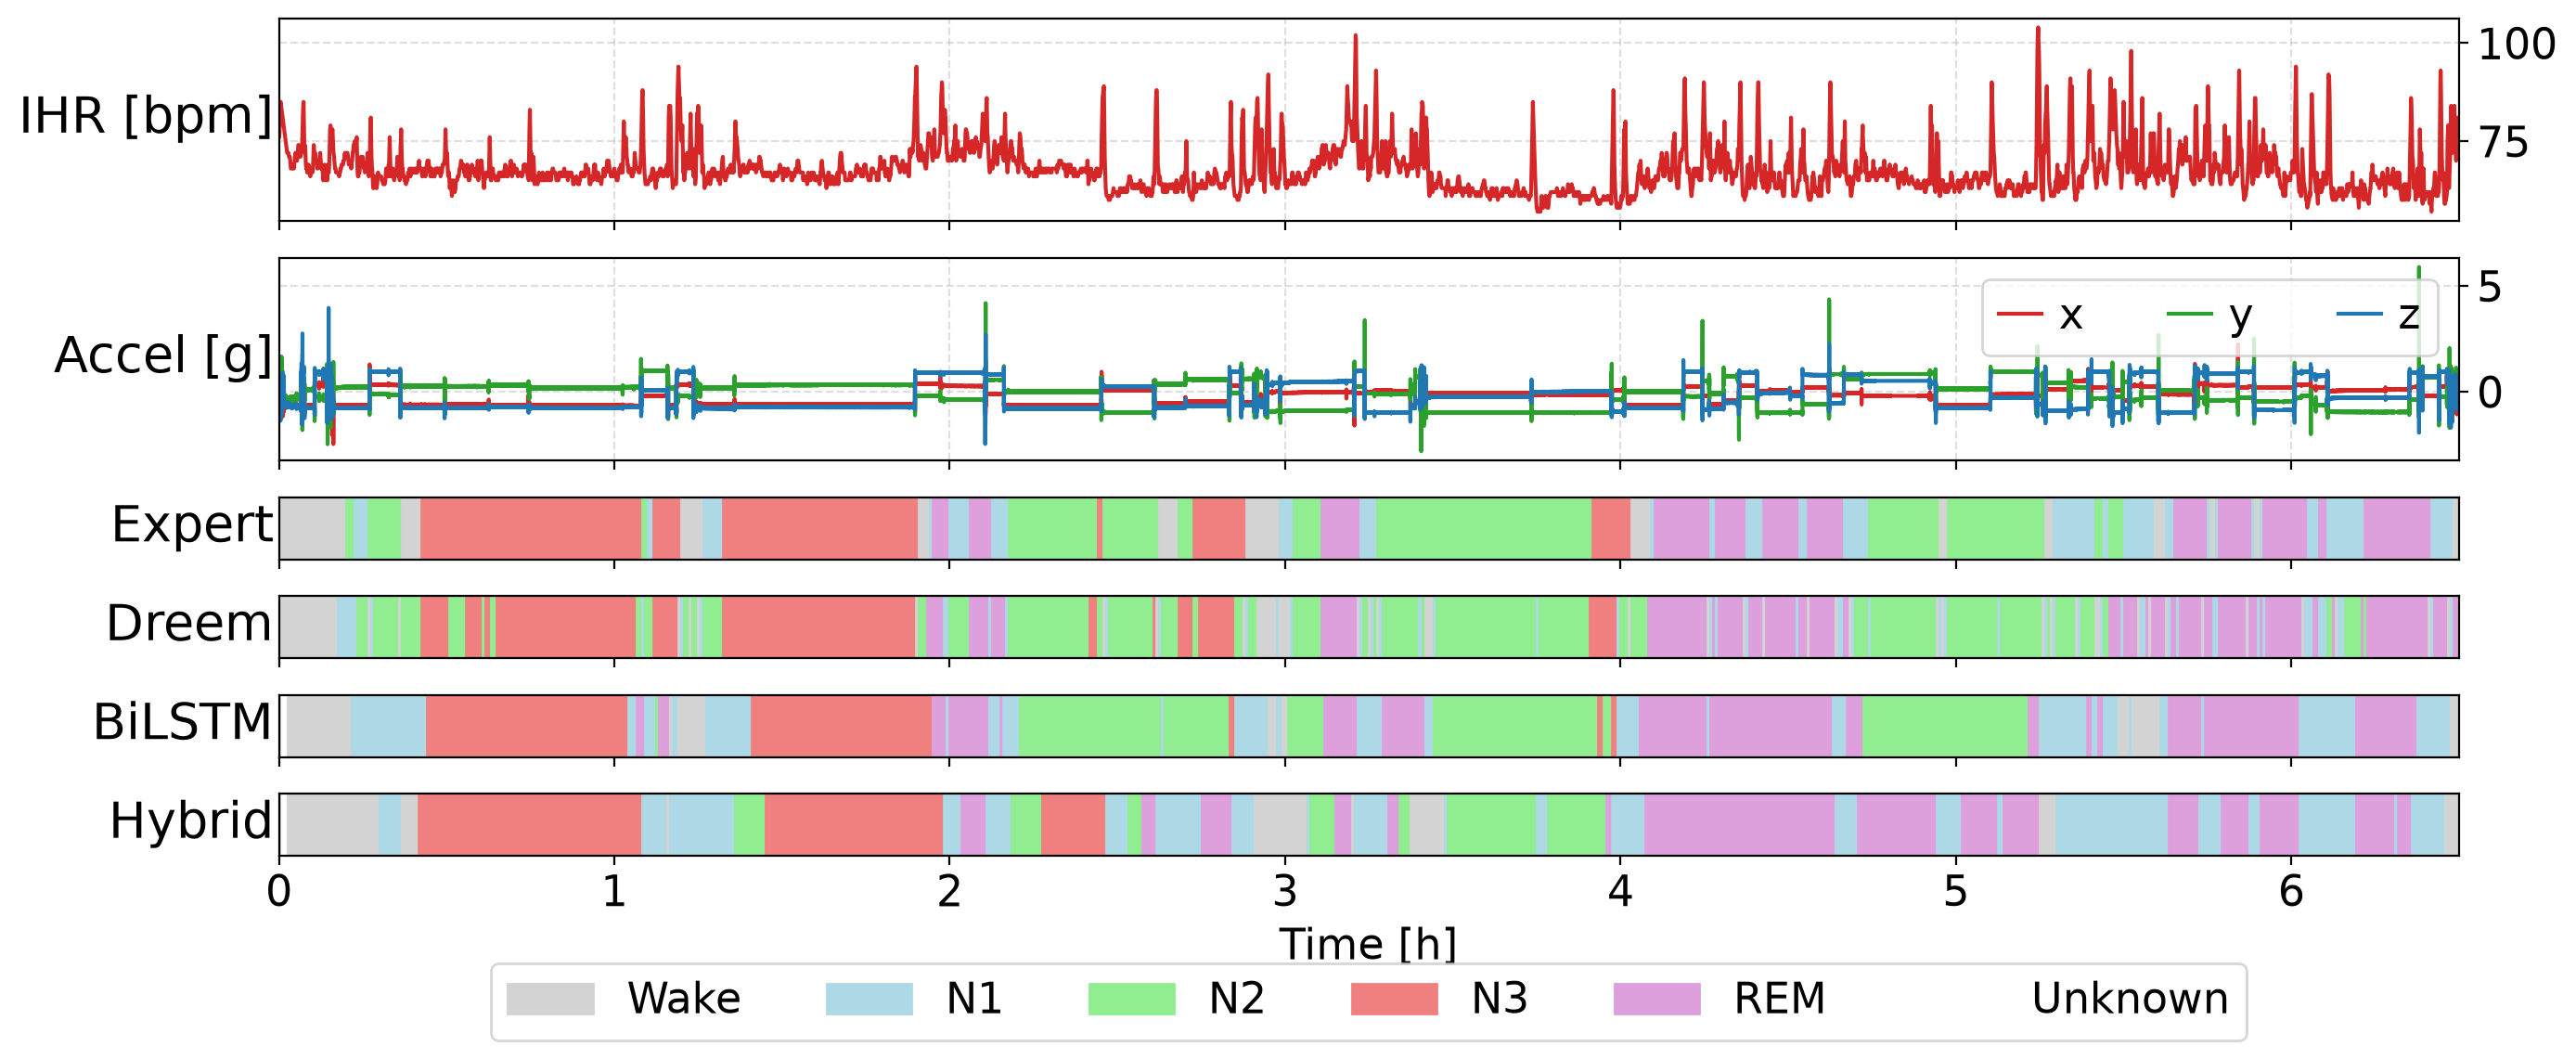
\includegraphics[width=\linewidth]{../report/figures/night-predictions-31-1.png}\\[1mm]
  \pnote{\itshape Paciente 31: la BiLSTM reproduce la macroestructura del hipnograma del experto
  —bloques de N2/Deep y REM al final—; el híbrido fragmenta más y sobre-predice Wake.}}

\block{Dónde falla · matriz de confusión BiLSTM (4 cl.)}{%
  \centering
  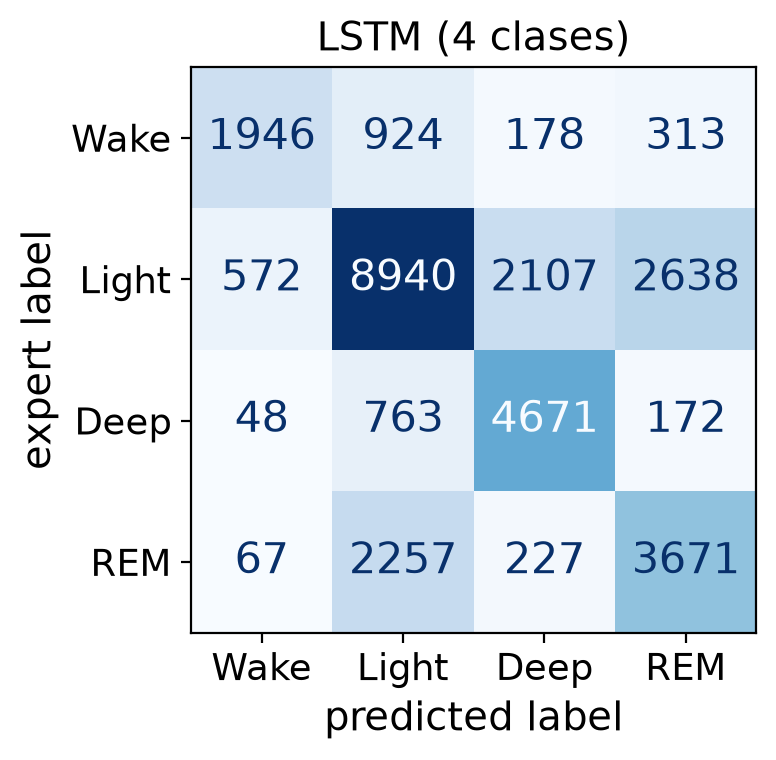
\includegraphics[width=0.82\linewidth]{../report/figures/lstm-confussion-4.png}\\[1mm]
  \pnote{\itshape Diagonal marcada; el error residual vive en la frontera Light--REM (sin EEG,
  REM $\approx$ sueño ligero). Deep es la mejor resuelta: IHR mínimo e inmovilidad.}}

\block{Apéndice · Interpretabilidad (SHAP)}{%
  \centering
  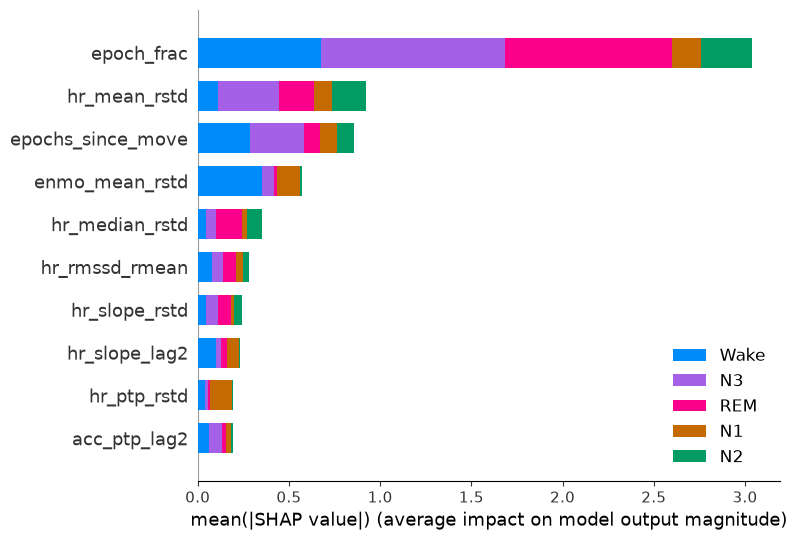
\includegraphics[width=\linewidth]{../report/figures/xgboost-shap.png}\\[1mm]
  \pnote{\itshape Importancia SHAP del XGBoost por etapa: dominan \texttt{epoch\_frac}, estadísticos
  móviles (\texttt{\_rstd}) y \texttt{epochs\_since\_move} — todas de contexto temporal.}}

\block{Conclusión \& trabajo futuro}{%
  Un pipeline completo de sleep staging desde la muñeca confirma que \textbf{la dependencia
  inter-época domina}. El híbrido no superó al enfoque tabular por el sobreajuste de su encoder
  entrenado de cero.\par\vspace{1.5mm}
  $\bullet$ \textbf{Intra-época:} preentrenamiento \textbf{auto-supervisado} (autoencoders) para un
  embedding más robusto.\\
  $\bullet$ \textbf{Inter-época:} sustituir la recurrencia por \textbf{auto-atención (Transformers)}.
  \par\vspace{1.5mm}
  \pnote{La referencia \textbf{SLAMSS-IFS} combina ambas y supera a nuestra BiLSTM por apenas
  $\sim$5\% de accuracy (4 clases).}}

\end{columns}

%======================= FRANJA DE CIERRE ==========================
\begin{columns}\column{1}
\begin{darkblock}
\block{Mensaje clave}{%
  \begin{minipage}[c]{0.60\linewidth}\color{ivory}\large
    Con solo una muñeca —sin EEG— y modelando la \textbf{secuencia de la noche}, una BiLSTM se acerca
    de forma razonable al techo humano. El límite ya no es el clasificador: es
    \textbf{\color{ambersoft}la señal}.
  \end{minipage}\hfill
  \begin{minipage}[c]{0.36\linewidth}\centering
    {\color{amber}\bfseries\fontsize{40}{40}\selectfont 0.46\quad0.57\quad0.84}\\[2mm]
    {\small\color{ivory} $\kappa$ vs. experto \quad\; F1 macro \quad\;\, AUC-ROC}
  \end{minipage}}
\end{darkblock}
\end{columns}

\end{document}
